\section{Analysing the data}
\label{sec:analysing_the_data}

\subsection{Launching Matlab}

Note that to launch the CITE app below one needs Matlab 2019a or a higher version. The KCM analysis part, instead, requires Matlab 2018a or a higher version.

Once Matlab is launched, one shall change the directory in the command window to the folder "Scripts" (cf.\ Figure~\ref{fig:file-structure-base-folder}). Once there, execute \texttt{main.m}.

\subsection{The initial prompt}

Launching \texttt{main.m} will initially produce a series of debug messages, and then a prompt like the one in Figure~\ref{fig:main-menu}.

\begin{figure}[!htbp]
	\centering
	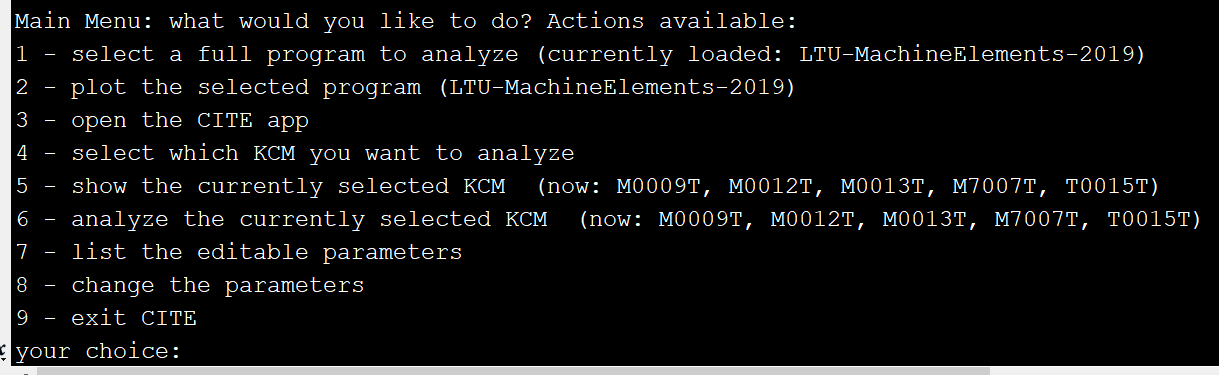
\includegraphics[width = 0.8\textwidth]{main-menu}
	\caption{Main menu that one obtains by launching \texttt{main.m}.}
	\label{fig:main-menu}
\end{figure}

The most interesting (and not self-explaining) items are:
%
\begin{itemize}
	\item ``plot the selected program'', that will produce a figure that summarizes which course connects with which other in terms of \acp{KC}. Note that the suite will assign all the prerequisite \acp{KC} that are not taught by any course to an artificial ``prerequisites'' course. Note also that the plot is explorable - in the sense that clicking on the various arrows will expand which \acp{KC} form the connections;
	\item ``open the CITE app'' - for this item see Section~\ref{ssec:the_cite_app};
	\item ``analyse the currently selected KCM'' - for this item see Section~\ref{ssec:the_kcm_analysis_prompt}.
\end{itemize}


\subsection{The KCM analysis prompt}
\label{ssec:the_kcm_analysis_prompt}

Selecting to analyse the currently selected KCM will produce a prompt like the one in Figure~\ref{fig:KCM-analysis-menu}.

\begin{figure}[!htbp]
	\centering
	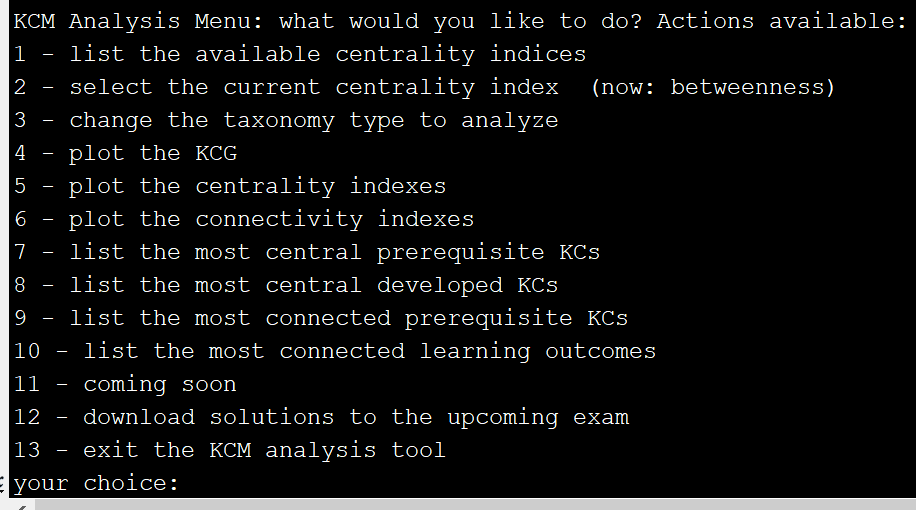
\includegraphics[width = 0.8\textwidth]{KCM-analysis-menu}
	\caption{Menu that one obtains by launching an analysis of the currently selected KCM.}
	\label{fig:KCM-analysis-menu}
\end{figure}

The most interesting (and not self-explaining) items are:
%
\begin{itemize}
	\item ``plot the KCG'', that will open the CITE app (thus check Section~\ref{ssec:the_cite_app} for this item);
	\item ``plot the centrality indexes'', that will produce a figure that should be interpreted as suggested in Section~\ref{sec:interpreting_the_results}.
\end{itemize}

\subsection{The CITE app}
\label{ssec:the_cite_app}

Once the app is launched, you will get a blank graph plot, and a list of courses on the right. Selecting the desired courses with the mouse (shift+click) and then pressing the ``Plot'' button will produce an other explorable plot. Here clicking on the various nodes will highlight connections. Different colors are also placeholders for different taxonomical levels. Clicking the ``Show Structural Problems'' item will moreover highlight structural issues in the \ac{KCG}, that may be either of a temporal structure (i.e., a course assumes that a prerequisite \ac{KC} has been taught, but it has actually been taught at a later course) or taxonomical level structure (i.e., one assumes that a prerequisite has been previously taught at a certain level, but actually it has been taught at a lower level).


